\documentclass{article}
\title{Statistics}
\date{November 18, 2019}
\usepackage{amsmath}
\usepackage{mathtools}
\usepackage{textcomp}
\usepackage{multicol}
\usepackage{fullpage}
\usepackage{graphicx}

\begin{document}
\maketitle

\section{Five Number Summary}
\begin{enumerate}
    \item $minimum$ - The Smallest Value
    \item $Q_1$ - The First Quartile -- the value such that 25\% of the cases are less than
        or equal to $Q_1$
    \item $median$ - The value such that 50\% of the cases are less
        than or equal to $median$ and 50\% of the cases are greater than
        or equal to $median$
    \item $Q_3$ - The Third Quartile -- the value such that 75\% of the cases are less than
        or equal to $Q_3$
    \item $maximum$ - The Largest Value
\end{enumerate}

\subsection{Computing the Five Number Summary}
\begin{enumerate}
    \item Sort your data in ascending order.
    \item Find the $minimum$ and $maximum$, these will be the numbers
        at the beginning and end of your sorted data.
    \item Find the $median$ by observing the value which divides the
        list in two.  If you have an even number of cases, average the
        two middle values.
    \item Find the $Q_1$ value by drawing brackets around the numbers
        that are less than the median.  Find the median of this set.
    \item Find the $Q_3$ value by drawing brackets around the numbers
        that are greater than the median. Find the median of this set.
\end{enumerate}

\subsection{Box Plots}
\begin{itemize}
    \item Boxplots are graphical representations of the five number
        summary.
    \item They give an idea of the distribution of cases.
    \item Plotting boxes side by allow us to compare sets of data.
\end{itemize}
\begin{center}
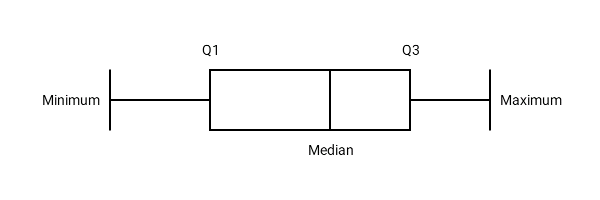
\includegraphics[height=1.5in]{images/Boxplot}
\end{center}
\pagebreak

\section{Mean}
\begin{itemize}
    \item The mean is another measure of center.
    \item The mean is the value each data item would hold if we evenly
        distributed the value across all the cases. (Like communism,
        but without the oppressive regimes!)
    \item The mean is computed by the formula:
    \[
        \bar{x} = \dfrac{1}{n} \displaystyle\sum_{i=1}^{n} x_i
    \]
    \item The variables in this (and other statistics calculations)
    are:
    \begin{itemize}
        \item $\bar{x}$ -- The Mean
        \item $X$ -- The Set of All Cases
        \item $x_i$ -- The $i^\mathrm{th}$ Case in $X$
        \item $n$ -- The Number of Cases in $X$
    \end{itemize}
\end{itemize}

\section{Measuring Spread About the Mean}
\begin{itemize}
    \item If we think of the mean as a measure of center, how can we
        measure  the spread about the mean?
    \item We may attempt to measure the average deviation from the
        mean:
        \[
            \dfrac{1}{n} \displaystyle\sum_{i=1}^{n} x_i - \bar{x}
        \]
    \item Let's try it out on the exam data!
    \item What happened? 
    \item Why do we get zero, or a number very close to it?
    \item We could fix this by squaring each difference (so now they
        are all positive)
        \[
            \dfrac{1}{n} \displaystyle\sum_{i=1}^{n} (x_i - \bar{x})^2
        \]
    \item Now, the problem becomes that we have the wrong units!  Why?
    \item So we correct this, and arrive at the \textbf{standard
        deviation}:
        \[
            \sigma = \sqrt{\dfrac{1}{n} \displaystyle\sum_{i=1}^{n}
            (x_i - \bar{x})^2}
        \]
    \item The above formula is the theoretical standard deviation, but
        is often biased toward extant data.  So we typically make the
        deviation a bit wider by decreasing the denominator by one:
        \[
            s = \sqrt{\dfrac{1}{n-1} \displaystyle\sum_{i=1}^{n}
            (x_i - \bar{x})^2}
        \]
    \item $\sigma$ is the population standard deviation and $s$ is the
        sample standard deviation.
    \item From now on, we will always use $s$.
    \item Let's compute $s$ for the exam data! What does $s$ tell us?
\end{itemize}

\end{document}
